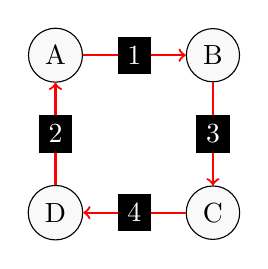
\begin{tikzpicture}
\node[shape=circle,draw=black,fill=gray!5] (D) at (0,0) {D};  \node[shape=circle,draw=black,fill=gray!5] (A) at (0, 2) {A};
\node[shape=circle,draw=black,fill=gray!5] (B) at (2, 2) {B};
\node[shape=circle,draw=black,fill=gray!5] (C) at (2, 0) {C};

\path [->] (A) edge[color=red,thick] (B);
\path [->] (B) edge[color=red,thick] (C);
\path [->] (C) edge[color=red,thick] (D);
\path [->] (D) edge[color=red,thick] (A);

\node[shape=rectangle, draw=black,fill=black, text=white] (4) at (1, 0) {4};
\node[shape=rectangle,draw=black,fill=black, text=white] (2) at (0, 1) {2};
\node[shape=rectangle,draw=black,fill=black, text=white] (1) at (1, 2) {1};
\node[shape=rectangle,draw=black,fill=black, text=white] (3) at (2, 1) {3};
\end{tikzpicture}